%-------------------------------------------------------------------------------
%                            BAB II
%               TINJAUAN PUSTAKA DAN DASAR TEORI
%-------------------------------------------------------------------------------

\chapter{TINJAUAN KEPUSTAKAAN}                

\section{Struktur Penyaluran Gas LPG 3 Kg}
\par Dalam pendistribusian gas elpiji ke masyarakat, sepenuhnya dilakukan oleh Pertamina dengan sistem \textit{close loop  supply chain}, yaitu suatu aliran produk mulai dari konsumen, kembali ke pabrik untuk diproses ulang kemudian kembali lagi ke konsumen sebagai barang baru.
\par Dalam alur distribusi LPG 3 Kg, pertama-tama gas LPG di produksi di Depot LPG. Kemudian dari Depot LPG di distribusi kan menuju SPPBE (Stasiun Pengisian dan Pengangkutan Bulk LPG ) yang dikelola oleh Pertamina dan pihak swasta, kemudian setelah itu paket LPG diterima oleh agen LPG dan selanjutnya sebagai ujung tombaknya akan di distribusikan ke sub agen atau pangkalan LPG. Sub agen LPG inilah yang berhubungan langsung dengan pengecer, warung atau juga konsumen. seperti pada \ref{penyaluran}.
\begin{figure}[H]
	\centering
	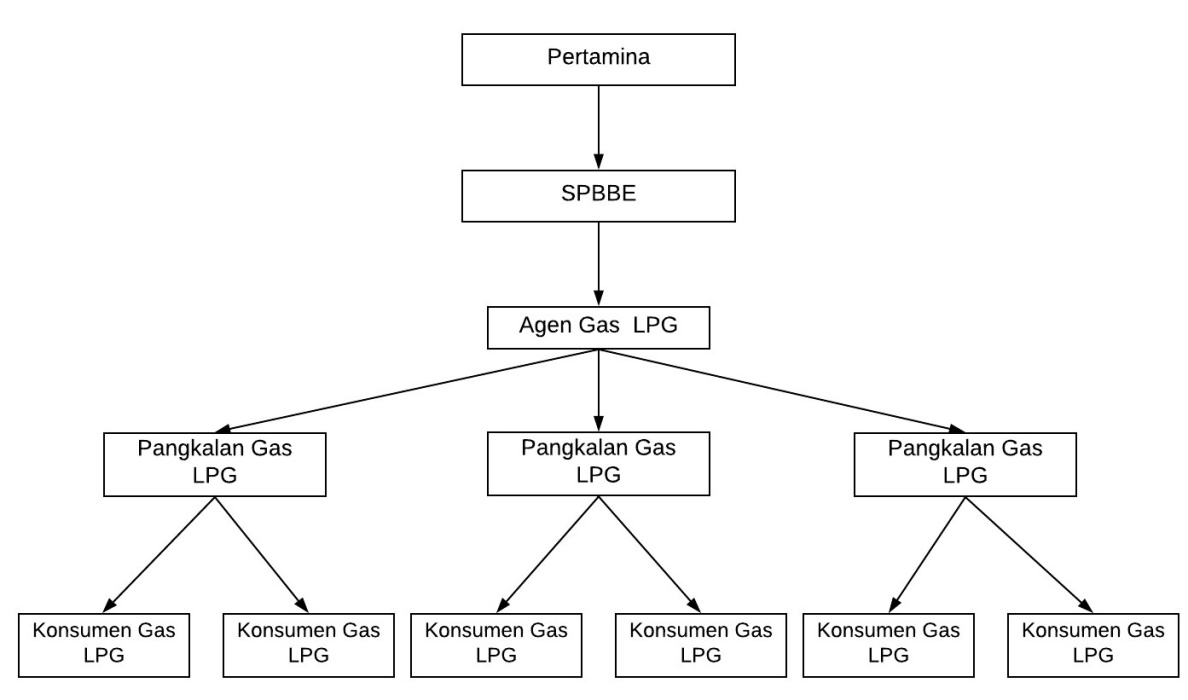
\includegraphics [width = 10cm, height= 10cm]{gambar/struktur-penyaluran}
	\caption{Struktur Penyaluran Gas LPG}
	\label{penyaluran}
\end{figure}


\section{Gas Subsidi LPG 3Kg}
\par Sejak Pemerintah melakukan konversi dari minyak tanah ke gas LPG yang dilakukan pada tahun 2007 menyebabkan kebutuhan untuk tabung gas LPG semakin meningkat dan gas subsidi LPG 3 kg yang ditawarkan pemerintah di awal periode konversi, semakin berkurang. Ini dikarenakan jenis tabung ini dianggap lebih ekonomis di bandingkan dengan tabung gas dan banyak rumah tangga dan industri rumahan kecil yang masih memakai tabung gas jenis ini sebagai alat untuk memasak.
\begin{figure}[H]
	\centering
	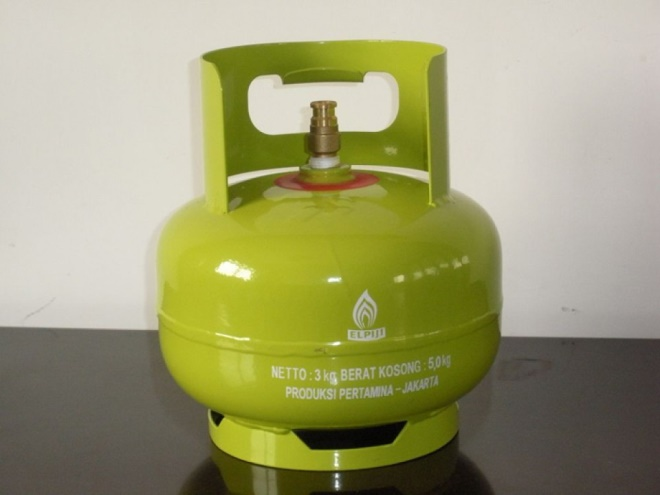
\includegraphics [width = 6cm, height= 8cm]{gambar/tabung-gas}
	\caption{Tabung Gas LPG}
	\label{tabung}
\end{figure}

\par Maka dari itu pertamina selaku distributor telah memberlakukan kebijakan kepada konsumen yang ingin membeli gas subsidi ini harus menunjukkan kartu keluarga (KK) dan Kartu Tanda Penduduk (KTP) sehingga jumlah tabung yang di beli dapat dibatasi berdasarkan KK.

\section{Android}
\par Android merupakan sistem operasi yang dibangun untuk perangkat mobile. Komponen-komponen dari sistem operasi Android ditulis dengan bahasa pemrograman C atau C++, akan tetapi aplikasi pengguna yang digunakan untuk Android ditulis dalam bahasa pemrograman Java \citep{ableson2012android}. Android juga dapat diartikan sebagai sistem operasi perangkat seluler berbasis Linux yang menyediakan run time environment yang disebut dengan \textit{Android Runtime} (ART) yang telah dioptimasi untuk perangkat dengan sistem memori yang kecil. Karena Android merupakan platform open source, maka setiap orang bebas untuk membuat dan mengembangkan suatu aplikasi \citep{supardi2011}.
%\begin{figure}[H]
%	\centering
%	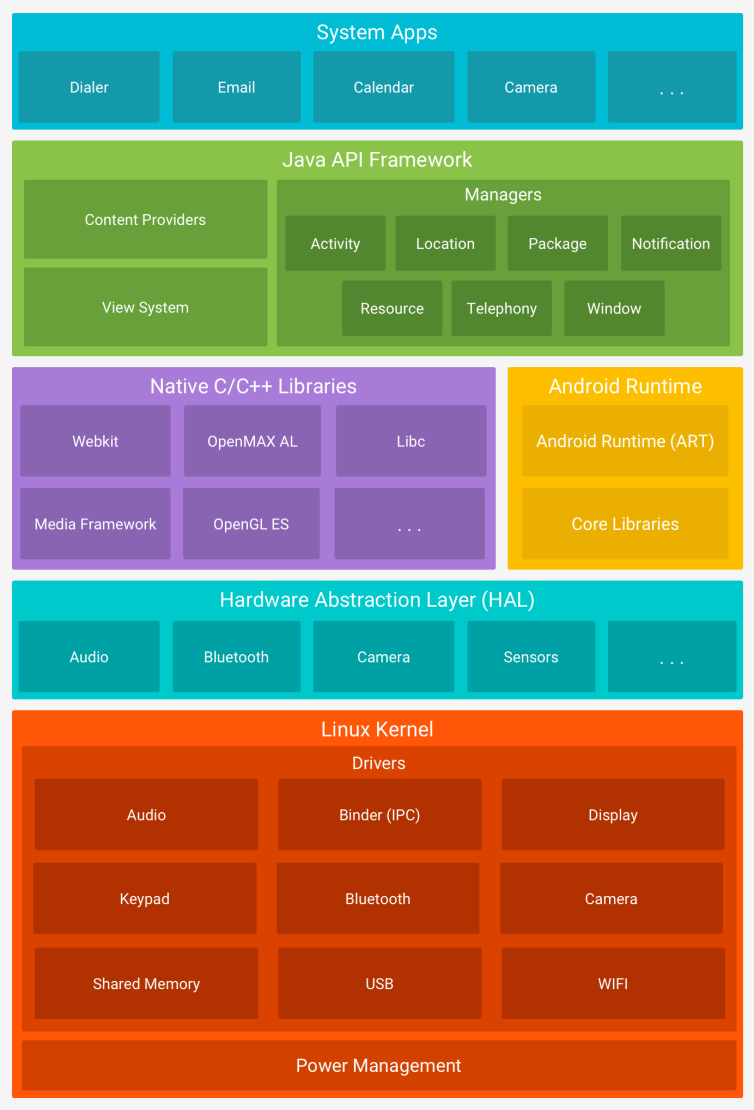
\includegraphics [width = 7cm, height= 6cm]{gambar/android}
%	\caption{Logo Android}
%	\label{android}
%\end{figure}



%-----------------------------------------------------------------------------%
\newpage
\section{Java}
Java pertama kali diluncurkan pada tahun 1995 sebagai bahasa pemrograman umum (\textit{general purpose programming language}) dengan kelebihan dia bisa dijalankan di web browser sebagai applet. Sejak awal, para pembuat Java telah menanamkan visi mereka ke dalam Java untuk membuat piranti-piranti yang ada di rumah (\textit{small embedded customer device}) seperti TV, telepon, radio, dan sebagainya agar dapat berkomunikasi satu sama lain. Karakteristik dari bahasa Java adalah sebagai berikut : \citep{Utama}
\begin{itemize}
	\itemsep0em
	\item Memiliki struktur Syntax yang sederhana
	\item Sangat berorientasi objek (OOP) dengan implementasi yang sangat baik sehingga
	kita bukan hanya belajar bagaimana membuat program yang baik (reusable,
	scalable, dan maintanable) tetapi juga kita belajar bagaimana cara berfikir yang
	baik untuk mengenali struktur masalah yang sedang kita hadapi.
	\item \textit{OpenPlatform}, \textit{Write Once Run Anywhere} (WORA), portabel atau \textit{multi platform}, program yang kita buat dapat dijalankan di Windows, Linux/Unix, Solaris, dan MacIntosh tanpa perlu diubah maupun di kompilasi ulang.
	\item Arsitekturnya yang kokoh dan pemrograman yang aman didukung oleh komunitas
	\textit{Open Source}
	\item Bukan sekedar bahasa tapi juga platform sekaligus arsitektur. Java mempunyai portabilitas yang sangat tinggi.
\end{itemize}

\section{Servlet}
Servlet merupakan salah satu modul perpustakaan yang ditulis dalam bahasa pemrograman Java yang berupa \textit{class} yang digunakan untuk merespon permintaan \textit{client}. Servlet tidak terikat dengan protokol client-server tertentu tetapi paling sering menggunakan protokol HTTP dan kata "Servlet" sering digunakan dalam arti "HTTP Servlet" \citep{servlet}. Penggunaan umum untuk HTTP Servlet meliputi:
\begin{itemize}
	\itemsep0em
	\item Memproses dan / atau menyimpan data yang dikirimkan oleh formulir HTML.
	\item Menyediakan konten dinamis, contohnya mengembalikan hasil kueri basis data ke klien.
	\item Mengelola informasi \textit{state} di dalam protokol \textit{stateless} HTTP.
\end{itemize}
\newpage
\section{Google App Engine}
Google App Engine (GAE) adalah layanan untuk mengembangkan dan hosting aplikasi Web di pusat data Google, yang termasuk ke dalam komputasi awan kategori Platform As Services (PaaS). Aplikasi web yang di jalankan pada GAE  dijalankan di beberapa server untuk redundansi dan memungkinkan penskalaan sumber daya sesuai dengan persyaratan trafik tertentu. App Engine secara otomatis akan mengalokasikan sumber daya tambahan ke server untuk mengakomodasi peningkatan beban. Kelebihan dari GAE adalah sebagai berikut: \citep{technopedia}
\begin{itemize}
	\itemsep0em
	\item Server yang tersedia tanpa memerlukan konfigurasi
	\item Power scaling yang menurunkan hingga ke tingkat "gratis" ketika saat penggunaan sumber daya minimal.
	\item Alat komputasi awan yang otomatis
\end{itemize}

\section{Aplikasi Hybrid (\textit{Mobile Hybrid App})}
Aplikasi hybrid adalah aplikasi web yang ditransformasikan menjadi kode native pada platform seperti iOS atau Android. Aplikasi hybrid biasanya menggunakan browser untuk mengijinkan aplikasi web mengakses berbagai fitur di device mobile seperti Push Notification, Contacts, atau Offline Data Storage. Beberapa tools untuk mengembangkan aplikasi hybrid antara lain Phonegap, Rubymotion dan lain-lain \citep{Permana}.
\begin{figure}[H]
	\centering
	\fbox{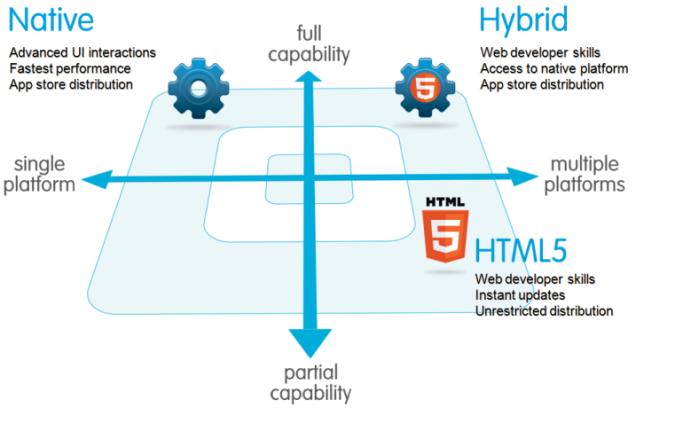
\includegraphics [width = 12cm, height= 8cm]{gambar/hybrid}}
	\caption{Perbandingan Aplikasi Native \& Hybrid}
	\label{android}
\end{figure}
\par Keuntungan membangun aplikasi hybrid diantaranya pemeliharaan project menjadi semakin mudah jika dibandingkan dengan aplikasi native. Aplikasi hybrid juga, bisa dibangun secara cepat untuk keperluan cross platform dan dana yang bisa menjadi lebih hemat jika dibandingkan dengan native.


\section{Ionic Framework}

Ionic adalah \textit{framework front-end} yang dikhususkan untuk membangun aplikasi \textit{hybrid} dengan HTML5, CSS dan AngularJS. Ionic menggunakan Node.js SASS, AngularJS sebagai \textit{engine}-nya. Ionic dilengkapi dengan komponen-komponen CSS seperti \textit{button, list, card, form, grids, tabs}, dan masih banyak lagi. Jadi Ionic itu merupakan teknologi web yang bisa digunakan untuk membuat suatu aplikasi \textit{mobile}. Karena \textit{hybrid} maka aplikasi hanya dibuat satu kali tetapi sudah bisa dirilis di lebih dari satu \textit{platform} dengan kata lain \textit{cross-platform} \citep{Wahyuni}.


\section{Apache Cordova}
\par Seperti yang telah dijelaskan di atas, bahwa Ionic hanya menyediakan \textit{framework Front-end} sedangkan untuk mengubahnya ke dalam \textit{platform} Android dan IOS, Ionic menggunakan Apache Cordova. Apache Cordova adalah \textit{platform} untuk membangun aplikasi \textit{mobile native} menggunakan HTML, CSS dan JavaScript. Native mobile application yang didukung antara lain Android, iOS, Windows Phone dan Blackberry.
\par Apache Cordova berisi sekumpulan API (\textit{Application Programming Interface}) untuk mengakses device dari perangkat mobile. Device itu antara lain kamera, GPS (\textit{Global Positioning System}), storage dan lain-lain.  Dengan menunggunakan UI (\textit{User Interface}) framework seperti jQuery Mobile, Dojo Mobile atau Sencha Touch, maka kita dapat mengakses API ini. Dengan kata lain kita dapat membangun aplikasi hanya menggunakan HTML, CSS dan Javascript.


\section{Angular}
\par Untuk melakukan implementasi logika, Ionic menggunakan teknologi framework javascript bernama Angular yang menawarkan performa dan respon cepat seperti aplikasi \textit{native}. sebelumnya dikenal dengan nama AngularJS, sekarang dikenal dengan nama Angular (tanpa JS dibelakang). Angular yang merupakan versi terkini dari AngularJS tentu masih banyak peminatnya di dunia pemrograman. Angular telah mengalami banyak sekali perubahan dibandingkan pendahulunya AngularJS. Angular kini sudah side by side dengan framework Javascript modern lainnya seperti React, Vue dan lain-lainnya. Secara konsep Angular sudah lumayan matang, dengan mampu mengakomodir component based dan dengan bergabungnya Typescript milik Microsoft dan RxJS milik ReactiveX untuk mendukung kemapanan framework ini. Performa yang dihasilkan oleh Angular kini bisa disejajarkan dengan para kompetitor dikelasnya.


\section{Metode Pengembangan Perangkat Lunak}
Pengembangan perangkat lunak dapat diartikan sebagai proses-proses yang dilakukan untuk memgembangkan suatu perangkat lunak yang baru atau memperbaiki perangkat lunak yang telah ada. Agar proses-proses tersebut berjalan lebih cepat, tepat, dan juga hasilnya mudah di kembangkan dan dipelihara, maka pengembangan perangkat lunak memerlukan suatu metodologi khusus. Metodologi Pengembangan Perangkat Lunak merupakan suatu proses pengelolaan kumpulan metode dan konvensi notasi yang telah didefinisikan untuk mengembangkan perangkat lunak. Metode pengembangan perangkat lunak secara prinsip bertujuan untuk membantu menghasilkan perangkat lunak yang berkualitas \citep{jauhari}. Komponen metodologi pengembangan perangkat lunak dapat dibagi dalam tiga unit, yaitu \citep{pressman2005software}:
\begin{enumerate}
	\item Metode, yaitu suatu cara atau teknik pendekatan yang sistematik yang dipergunakan untuk mengembangkan perangkat lunak. Metode ini mencakup : Perencanaan proyek dan  perkiraan, analisis keperluan sistem dan perangkat lunak, perancangan struktur data, arsitektur program, prosedur algoritma, Coding, uji coba dan pemeliharaan.
	\item Alat bantu (\textit{Tools}), yaitu alat-alat (manual atau otomatis) yang mendukung pengembangan  perangkat lunak. Terdapat 2 alat Bantu yang dapat digunakan yaitu : alat Bantu manual dan alat Bantu otomatis.
	\item Prosedur, yang dipergunakan untuk mendefinisikan urut-urutan pekerjaan (siklus) dari metode dan alat bantu tersebut.
\end{enumerate}

\section{Scrum}
Scrum adalah bagian dari metode Agile yang dirancang untuk menambah fokus, kejelasan dan transparansi pada perencanaan dan implementasi proyek. Agile sendiri merupakan pendekatan pengembangan perangkat lunak yang mengutamakan pada kesiapan untuk melakukan perubahan pada tahap pengembangan perangkat lunak \citep{raharjana2017pengembangan}. Scrum digunakan dalam perusahaan perangkat lunak kecil, menengah dan besar di seluruh dunia. Kelebihan dari metode pengembangan perangkat lunak menggunakan Scrum adalah sebagai berikut: 
\begin{itemize}
	\itemsep0em
	\item Meningkatkan kecepatan proses pengembangan.
	\item Menyamakan tujuan individu dan perusahaan.
	\item Menciptakan budaya yang didorong oleh kinerja.
	\item Mendukung pembuatan nilai pemegang saham.
	\item Tercapainya komunikasi kinerja yang stabil dan konsisten di semua tingkatan.
	\item Meningkatkan pengembangan individu dan kualitas hidup
\end{itemize}

\par Komponen utama dari Scrum adalah tim Scrum dan peran, acara, dan artefak yang terkait dengannya. tim Scrum terdiri dari 3 peran yaitu \textit{Product Owner}, \textit{Scrum Master} dan \textit{Development Team}. \textit{Product Owner} adalah satu-satunya orang yang bertanggung jawab dalam pengelolaan Product Backlog. \textit{Development Team} dibentuk dan diberikan wewenang oleh organisasi untuk menyusun dan mengelola pekerjaan mereka sendiri. \textit{Scrum Master} bertanggung jawab untuk mengenalkan dan menyokong penggunaan Scrum sebagaimana dijelaskan di dalam Panduan Scrum ini. \textit{Scrum Master} melakukan ini dengan membantu orang-orang agar dapat memahami teori, praktik-praktik, aturan-aturan dan tata nilai Scrum. Scrum memiliki beberapa artefak-artefak atau dokumen yang merepresentasikan pekerjaan atau nilai bisnis guna terciptanya transparansi dan kesempatan untuk menginspeksi dan mengadaptasi. artefak-artefak terdiri dari Product Backlog dan Sprint Backlog.

\par \textit{Product Backlog} adalah daftar terurut dari seluruh fitur, fungsi, kebutuhan, peningkatan, dan perbaikan yang perlu diberlakukan terhadap produk pada rilis mendatang. Product Backlog item memiliki atribut deskripsi, urutan, estimasi dan nilai bisnis. Sedangkan, \textit{Sprint Backlog} adalah daftar item pada \textit{Product Backlog} yang terpilih untuk Sprint ditambah perencanaan untuk menghantarkan \textit{Increment} dan mencapai Sprint Goal. 

\par Scrum memiliki beberapa acara yang wajib dilakukan oleh seluruh anggota tim Scrum yaitu \textit{Sprint, Sprint Planning, Daily Scrum, Sprint Review, Sprint Retrospective}. Bagian terpenting dari Scrum adalah \textit{Sprint}, yaitu sebuah batasan waktu dengan durasi satu bulan atau kurang, dimana terdapat proses pembuatan \textit{Increment} yang dianggap “Selesai”. \textit{Increment} sendiri merupakan kumpulan item pada \textit{Product Backlog} yang diselesaikan dalam \textit{Sprint} dan total nilai bisnis \textit{Increment} dari seluruh \textit{Sprint} yang lalu.

\par \textit{Sprint Planning} adalah proses untuk merencanakan pekerjaan yang akan dikerjakan di \textit{Sprint}. Perencanaan ini dilakukan secara kolaboratif oleh seluruh anggota tim Scrum. \textit{Sprint Planning} memiliki batasan waktu maksimal delapan jam untuk Sprint yang berdurasi satu
bulan. \textit{Daily Scrum} adalah acara untuk \textit{Development Team} yang memiliki batasan waktu 15 menit. Dilakukan setiap hari selama Sprint berlangsung. \textit{Development Team} akan membuat rencana kerja untuk 24 jam ke depan. Acara ini mengoptimalkan kolaborasi dan performa dari tim dengan melakukan inspeksi pada pekerjaan yang dilakukan semenjak Daily Scrum sebelumnya.

\par \textit{Sprint Review} diselenggarakan di akhir setiap \textit{Sprint} untuk menginspeksi \textit{Increment} dan mengadaptasi \textit{Product Backlog} bila diperlukan. Pada saat \textit{Sprint Review}, tim Scrum dan pemegang kepentingan berkolaborasi untuk meninjau apa yang sudah   diselesaikan di Sprint. \textit{Sprint Retrospective} diselenggarakan setelah \textit{Sprint Review} dan sebelum \textit{Sprint Planning} berikutnya. Acara ini diselenggarakan paling lama tiga jam untuk Sprint yang berdurasi satu bulan. Untuk \textit{Sprint} yang lebih singkat, durasi acara ini biasanya lebih singkat \citep{panduanScrum}. Tujuan dari \textit{Sprint Retrospective} adalah:
\begin{itemize}
	\itemsep0em
	\item Melakukan inspeksi bagaimana jalannya Sprint terakhir yang terkait dengan orang-orang, hubungan antar mereka, proses, dan alat-alat yang digunakan.
	\item Melakukan identifikasi dan mengurutkan hal utama yang berjalan dengan baik dan peningkatan yang berpotensi untuk dilakukan.
	\item Membuat perencanaan untuk implementasi peningkatan cara kerja tim Scrum.
\end{itemize}
 

\section {\textit{Test Plan}}
\par Test Plan merupakan dokumen yang berisi definisi tujuan dan sasaran pengujian dalam lingkup iterasi (atau proyek), item-item yang menjadi target pengujian, pendekatan yang akan diambil, sumber daya yang dibutuhkan dan point untuk diproduksi. Dengan kata lain test plan dapat disebut sebagai perencanaan atau skenario untuk melakukan testing yang akan dilakukan baik oleh expert atau user umum. 
\par Tujuan umum membuat test plan secara umum adalah untuk memudahkan developer untuk melakukan testing agar testing yang dilakukan menjadi jelas sehingga hasilnya lebih berguna dan efisien. Tentunya dalam proses pembuatan test plan ini memerlukan beberapa langkah seperti berikut : \citep{guru99}
\begin{itemize}
	\item {Melakukan Analisa Produk}
	\newline Pada tahap ini kita harus meneliti seluruh bagian dari produk dan  meninjau dokumentasi dari produk. meninjau dokumentasi produk akan membantu memahami semua fitur-fitur dalam produk tersebut
	
	\item {Mengembangkan Strategi Pengujian}
	\newline Strategi pengujian adalah langkah yang penting saat membuat \textit{test plan}. berikut tahapan membuat strategi pengujian :
	\newpage
	\begin{itemize}
		\itemsep0em
		\item Mendefinisikan cakupan dari pengujian
		\item Mengidentifikasi Jenis Pengujian
		\item Dokumentasikan Resiko dan Masalah
		\item Menyiapkan Logistik Pengujian
	\end{itemize}
	
	\item {Mendefinisikan Objektif Pengujian}
	\newline Objektif Pengujian adalah keseluruhan tujuan dan pencapaian dari pelaksanaan pengujian. Tujuan pengujian ini adalah menemukan sebanyak mungkin cacat pada produk dan memastikan bahwa produk yang diuji bebas dari bug sebelum dirilis.
	
	\item Mendefinisikan Kriteria Pengujian
	\newline kriteria pengujian merupakan standar atau aturan yang prosedur atau penilaian pengujian dapat didasarkan. Ada 2 jenis kriteria pengujian yaitu sebagai berikut :
	\begin{itemize}
		\itemsep0em
		\item \textit{Suspension Criteria} : apabila kriteria ini terpenuhi maka siklus pengujian akan ditunda sampai permasalahan telah selesai
		\item \textit{Exit Criteria} : target persentase dari hasil pengujian yang dibutuhkan sebelum dilanjutkan ke tahap pengembangan selanjutnya
	\end{itemize}

	\item {Merencanakan Sumber Daya}
	\newline Rencana sumber daya merupakan ringkasan rinci dari semua jenis sumber daya yang dibutuhkan untuk menyelesaikan tugas proyek. Sumber daya dapat berupa manusia, peralatan dan material yang dibutuhkan untuk menyelesaikan proyek.
	
	\item Merencanakan Lingkungan Pengujian
	\newline Lingkungan pengujian adalah pengaturan perangkat lunak dan perangkat keras yang akan digunakan tim pengujian untuk melakukan uji coba. Lingkungan pengujian terdiri dari lingkungan bisnis dan pengguna yang nyata, serta lingkungan fisik, seperti server, lingkungan yang menjalankan ujung depan.
	
	\item {Melakukan Penjadwalan dan Estimasi}
	 \newline Dengan membuat jadwal yang padat dalam Perencanaan Pengujian, Manajer Pengujian dapat menggunakannya sebagai alat untuk memantau kemajuan dari proyek, mengendalikan pembengkakan biaya.
	 
	 \item {\textit{Test Deliverables}}
	 \newline \textit{Test Deliverables} adalah daftar semua dokumen, alat, dan komponen lain yang harus dikembangkan dan dipelihara untuk mendukung upaya pengujian.
	
\end{itemize}

\section {\textit{Usability Testing}}
\par \textit{Usability Testing} atau tes produk merupakan metode riset untuk mengembangkan dan menyempurnakan produk baru maupun yang telah ada. Inti dari riset ini adalah mendudukkan pengguna/pelanggan di pusat, lalu mengambil pelajaran dari sana. maka dalam test ini, mutlak adanya pengamatan secara langsung \citep{nielsen2012}
\par Dengan mendokumentasikan pengalaman aktual para calon pengguna aplikasi/produk dapat dievealuasi, sebab dari uji ini diharapkan akan menangkap kekuatan dan kelemahan dari setiap aspek yang ada pada aplikasi itu sendiri.

\section {\textit{Unit Testing}}
\textit{Unit Testing} adalah metode verifikasi perangkat lunak di mana programmer menguji suatu unit program layak untuk tidaknya dipakai. Unit testing ini fokusnya pada verifikasi pada unit yang terkecil pada desain perangkat lunak (komponen atau modul perangkat lunak). Karena dalam sebuah perangkat lunak banyak memiliki unit-unit kecil maka untuk mengujinya biasanya dibuat program kecil atau main program) untuk menguji unit-unit perangkat lunak. Unit-unit kecil ini dapat berupa prosedur atau fungsi, sekumpulan prosedur atau fungsi yang ada dalam satu file jika dalam pemrograman terstruktur, atau kelas, bisa juga kumpulan kelas dalam satu package. \citep{feridi}

%-----------------------------------------------------------------------------%

% Baris ini digunakan untuk membantu dalam melakukan sitasi
% Karena diapit dengan comment, maka baris ini akan diabaikan
% oleh compiler LaTeX.
\begin{comment}
\bibliography{daftar-pustaka}
\end{comment}
